
\section{Einführung}
\label{sec:Einfuehrung}
Für die ersten Praktikumstage ist es notwendig sich als erstes mit dem Wasserphantom zu beschäftigen. Dieses dient vor allem als Einstieg ins Bestrahlungsprogramm. Hierbei wird gelernt wie die Software Eclipse für die Bestrahlungsplanung funktioniert.  Die ersten wichtigsten Aufgaben sind vor allem die Erstellung eines Wasserphantoms, die Untersuchung von Dosisprofilen und  die Erstellung einer Tiefendosiskurve.


\section{Wasserphantom Teil 1}
\label{sec:Wasserphantom1}

\subsection{Erstellen eines Wasserphantoms}
\label{subsec:Erstellen}
Im ersten Teil soll das Programm kennengelernt werden.
Hierbei wird ein neuer "Patient" kreiert und im Konturierungsmodul soll ein Wasserphantom mit den Maßen $\SI{10}{\centi\meter}$ x $\SI{10}{\centi\meter}$ x $\SI{10}{\centi\meter}$, einem Schichtabstand von $\SI{0.25}{\centi\meter}$ und einem CT-Wert von Wasser erstellt werden.

\subsection{Erstellen eines PTVs}
\label{subsec:ErstellenPTV}
Im Zentrum des Phantoms wird eine kugelförmige Figur bzw. ein PTV mit einem Durchmesser von $\SI{5}{\centi\meter}$. Hier soll das PTV auch einen CT-Wert von Wasser besitzen.

\subsection{Erstellen eines Bestrahlungsplanes}
\label{subsec:Erstellenbestrahlung}
Als nächstes wird ein Bestrahlungsplan angelegt. Nun wird hier ein Bestrahlungsfeld mit den Maßen $\SI{5,5}{\centi\meter}$ x $\SI{5,5}{\centi\meter}$ und einer Photonenenergie von $\SI{6}{\mega\electronvolt}$ hinzugefügt. Außerdem soll hier die Gantry-Rotation den Wert 0$^\circ$ betragen, d.h. das Wasserphantom wird bei einer Gantry-Rotation von 0$^\circ$ bestrahlt.

\subsection{Berechnung der Dosisverteilung}
\label{subsec:Dosisverteilung}
Im nächsten Teil soll dann die Dosisverteilung berechnet werden. Dies geschieht mit Hilfe einem Algorithmus, der in diesem Fall mit AAA-CAP137 bezeichnet und in diesem Fall ausgewählt wird.

\subsection{Inverse Bestrahlungsplanung}
\label{subsec:inversebestrahlung}
Als Hilfe werden in diesem Aufgabenteil drei unterschiedliche Dosisverteilung in der Anleitung hinzugefügt. Diese sollen mit Hilfe des Bestrahlungsplanungsprogramms invers rekonstruiert werden. In diesem Fall sollen die Felder die Größe $\SI{5,5}{\centi\meter}$ x $\SI{5,5}{\centi\meter}$ und eine Photonenenergie von $\SI{6}{\mega\volt}$ besitzen.

\subsubsection{Erste Dosisverteilung}
In der Abbildung \ref{fig:ersteverteilung} ist die erste Dosisverteilung zu sehen. Die Dosisverteilung wird mit Hilfe von vier gleich gewichteten Strahlenfelder erzeugt und jedes Strahlenfeld besitzt eine Gantry-Rotation von $0^\circ$, $90^\circ$, $180^\circ$ und $270^\circ$. Das PTV befindet sich in der Mitte des Wasserphantoms. Die Strahlenfelder werden in diesem Fall mit MLCs für das PTV ausgerichtet. Dabei werden die MLCs mit einem Sicherheitssaum von $\SI{0.5}{\centi\meter}$ an das PTV angepasst. Die gegebene Dosisverteilung ist in der Abbildung \ref{abb:ersteverteilung} gezeigt.

\begin{figure}[H]
	\centering
	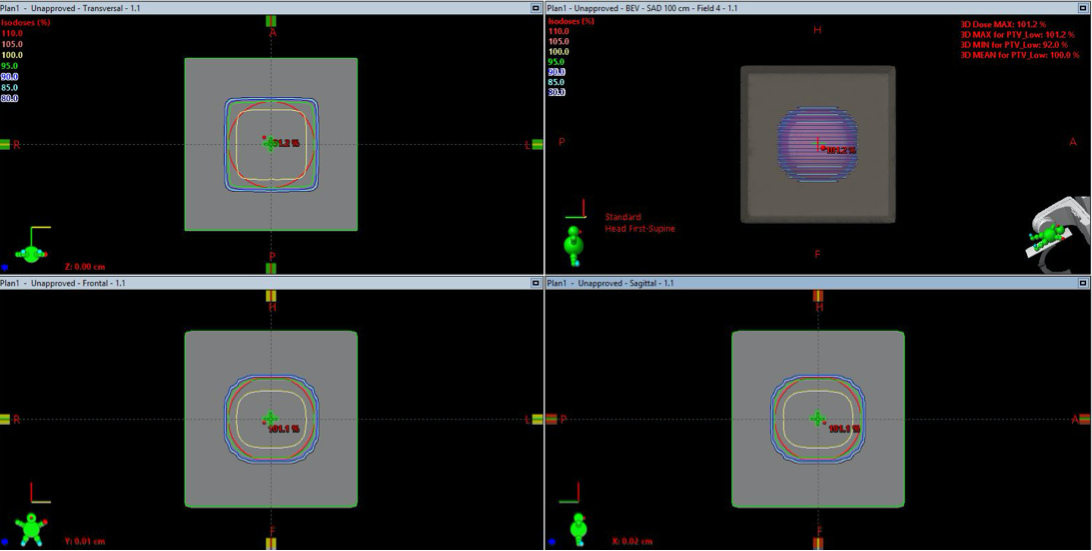
\includegraphics[width=0.7\linewidth]{../../Wasserphantom Bilder/AnleitungersteVerteilung.png}
	\caption{Darstellung der in der Anleitung gegebenen Dosisverteilung. \cite{Anleitung}}
	\label{abb:ersteverteilung}
\end{figure}

\begin{figure}[H]
	\centering
	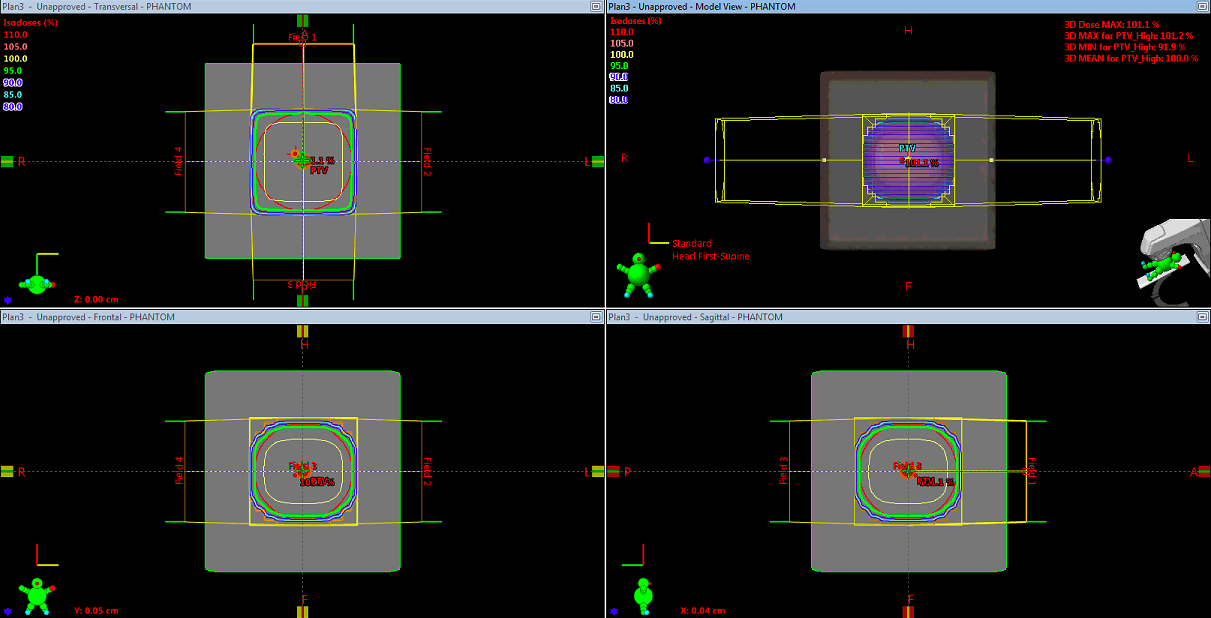
\includegraphics[width=0.7\linewidth]{../../Wasserphantom Bilder/ersteVerteilung.png}
	\caption{Die erste rekonstruierte Dosisverteilung.}
	\label{fig:ersteverteilung}
\end{figure}

\subsubsection{Zweite Dosisverteilung}
In der Abbildung \ref{fig:zweiteverteilung} ist die zweite Dosisverteilung zu sehen. Im Gegensatz zu dem anderen Aufgabenteil haben hier die Strahlenfelder eine Gantry-Rotation von $0^\circ$, $90^\circ$ und $225^\circ$. Dabei ist die Gewichtung des Feldes bei $0^\circ$ $32.5\%$, die des Feldes bei $90^\circ$ $34.5\%$ und die des Feldes bei $225^\circ$ $33\%$. Hierbei ergibt sich eine asymmetrische Form der Dosisverteilung, die mit der in der Anleitung gegebenen übereinstimmt (vgl. Abbildung \ref{abb:zweiteverteilung}).

\begin{figure}[H]
	\centering
	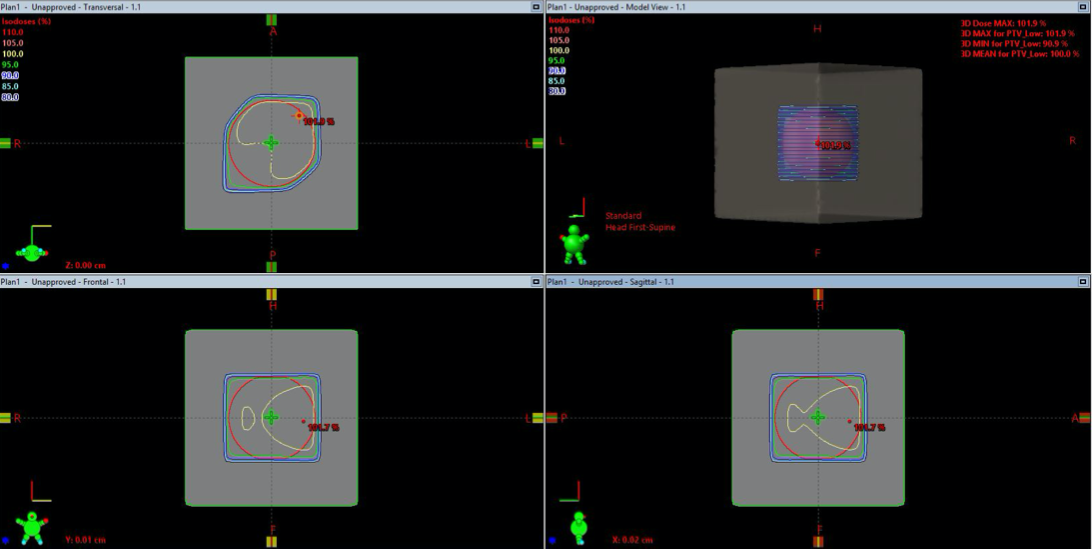
\includegraphics[width=0.7\linewidth]{../../Wasserphantom Bilder/AnleitungzweiteVerteilung.png}
	\caption{Darstellung der in der Anleitung gegebenen Dosisverteilung. \cite{Anleitung}}
	\label{abb:zweiteverteilung}
\end{figure}

\begin{figure}[H]
	\centering
	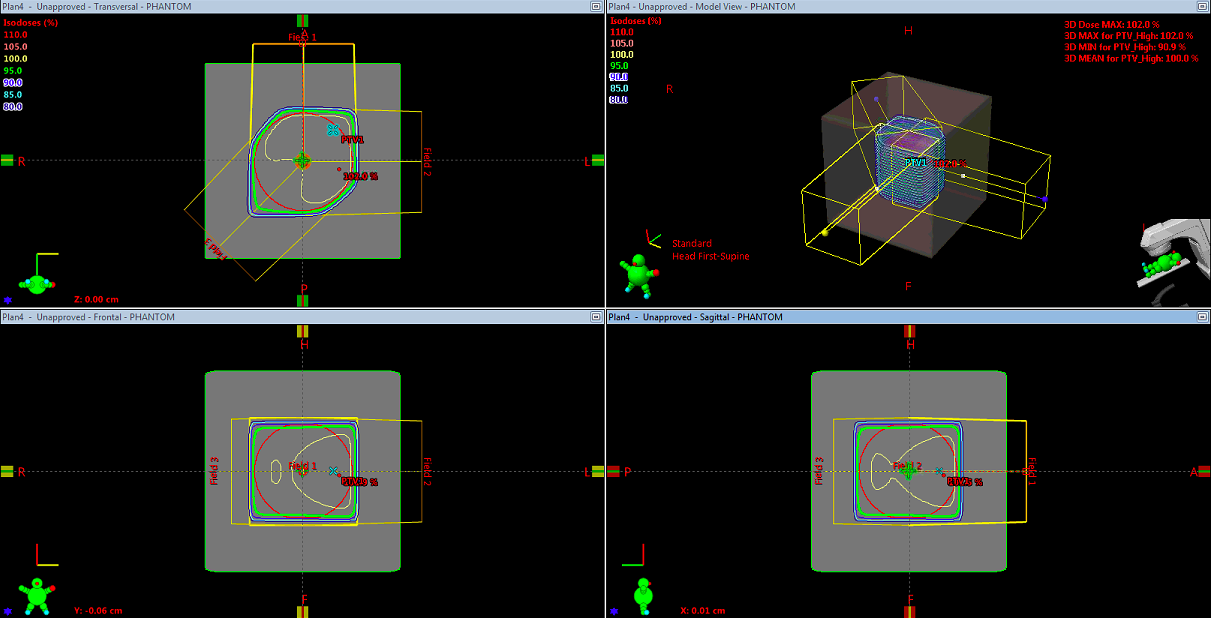
\includegraphics[width=0.7\linewidth]{../../Wasserphantom Bilder/zweiteVerteilung.png}
	\caption{Die zweite rekonstruierte Dosisverteilung.}
	\label{fig:zweiteverteilung}
\end{figure}

\subsubsection{Dritte Dosisverteilung}
In der Abbildung \ref{fig:dritteverteilung} ist die dritte Dosisverteilung zu sehen. Wie im vorherigen Teil handelt es sich hier auch um eine asymmetrische Form. Es ähnelt einem Hexagon. In diesem Fall wurden 6 Strahlenfelder bei Gantry-Rotationen von $30°$, $90°$, $150°$, $210°$, $270°$ und $330°$ verwendet. In diesem Fall sind alle Strahlenfelder gleichgewichtet.
Die gegebene Verteilung ist zum Vergleich in Abbildung \ref{abb:dritteverteilung}
dargestellt.

\begin{figure}[H]
	\centering
	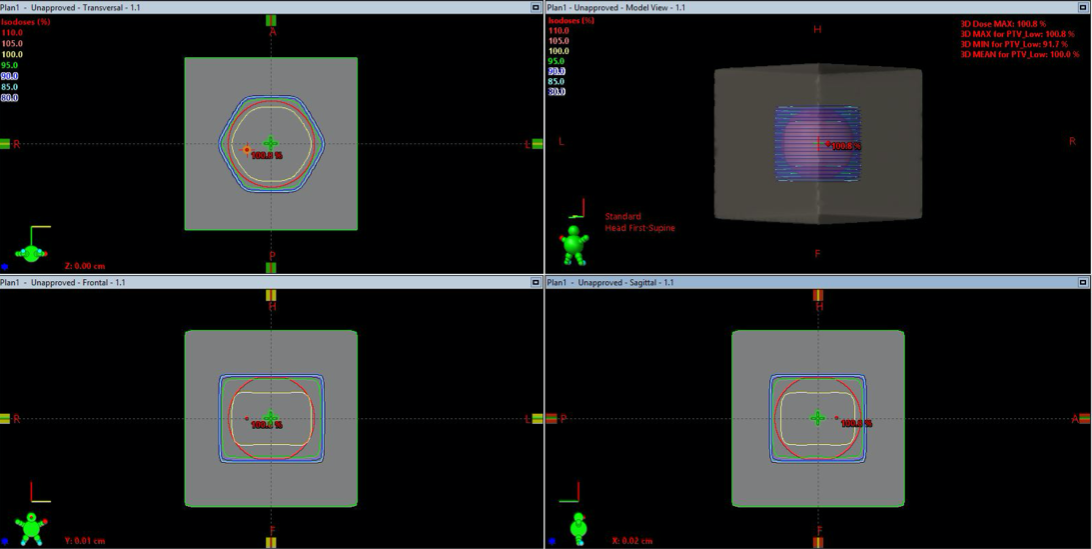
\includegraphics[width=0.7\linewidth]{../../Wasserphantom Bilder/AnleitungdritteVerteilung.png}
	\caption{Darstellung der in der Anleitung gegebenen Dosisverteilung. \cite{Anleitung}}
	\label{abb:dritteverteilung}
\end{figure}

\begin{figure}[H]
	\centering
	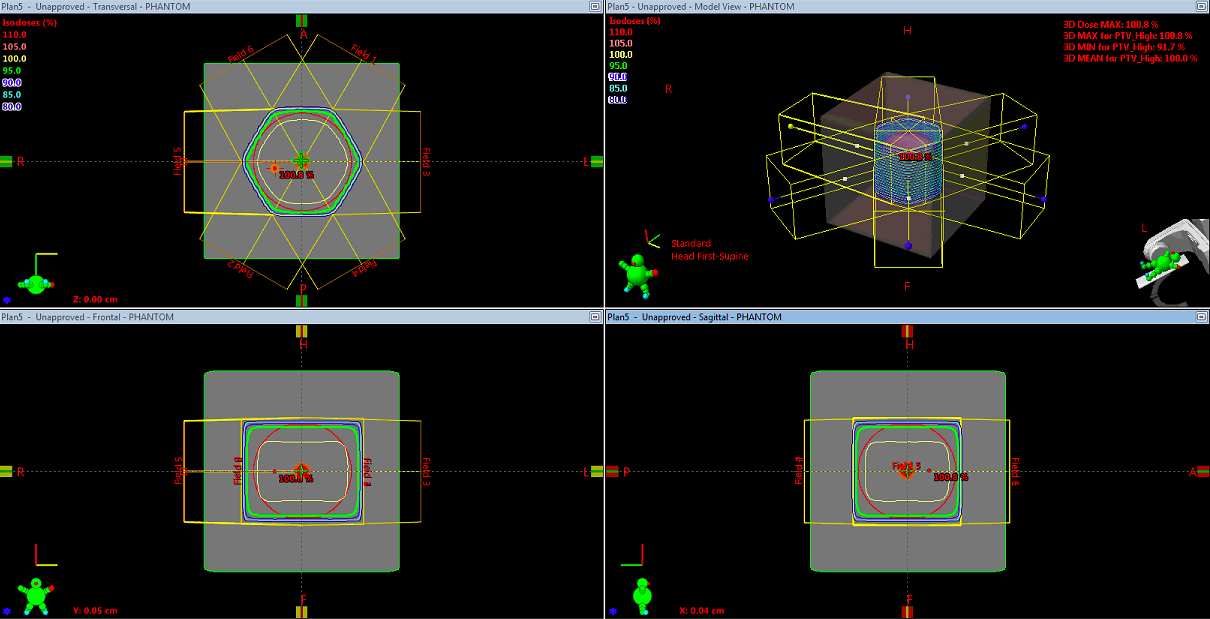
\includegraphics[width=0.7\linewidth]{../../Wasserphantom Bilder/dritteVerteilung.png}
	\caption{Die dritte rekonstruierte Dosisverteilung.}
	\label{fig:dritteverteilung}
\end{figure}


\section{Wasserphantom Teil 2}
\label{sec:Wasserphantom2}

\subsection{Untersuchung von Dosisprofilen}
\label{subsec:Dosisprofilen}

Zuerst soll ein Wasserphantom mit den Maßen $\SI{30}{\centi\meter}$ x $\SI{30}{\centi\meter}$ x $\SI{30}{\centi\meter}$, einem Schichtabstand von $\SI{0.25}{\centi\meter}$ und einem CT-Wert von Wasser erstellt werden. In das Zentrum des Wasserphantom wird eine Kugel mit dem Durchmesser von $\SI{5}{\centi\meter}$ als PTV definiert. Außerdem wird eine Gantry-Rotation von 0$^\circ$ verwendet und ein Strahlenfeld der Größe $\SI{10}{\centi\meter}$ x $\SI{10}{\centi\meter}$
mit einer Photonenenergie von $\SI{6}{\mega\volt}$. Das ist in der Abbildung \ref{fig:aufgabe21} zu sehen.
Das Strahlenfeld wird in der Tiefe des Phantoms breiter.
Der Referenzpunkt wurde in die Mitte des Wasserphantoms gesetzt, da dort auch das Zentrum des PTVs liegt. An diesem Punkt hat das Feld die eingestellte Feldgröße erreicht. Die Feldgröße hat aber eine Ungenauigkeit, die von der Auflösung und Schichtdicke des CTs abhängig ist.

\begin{figure}[H]
	\centering
	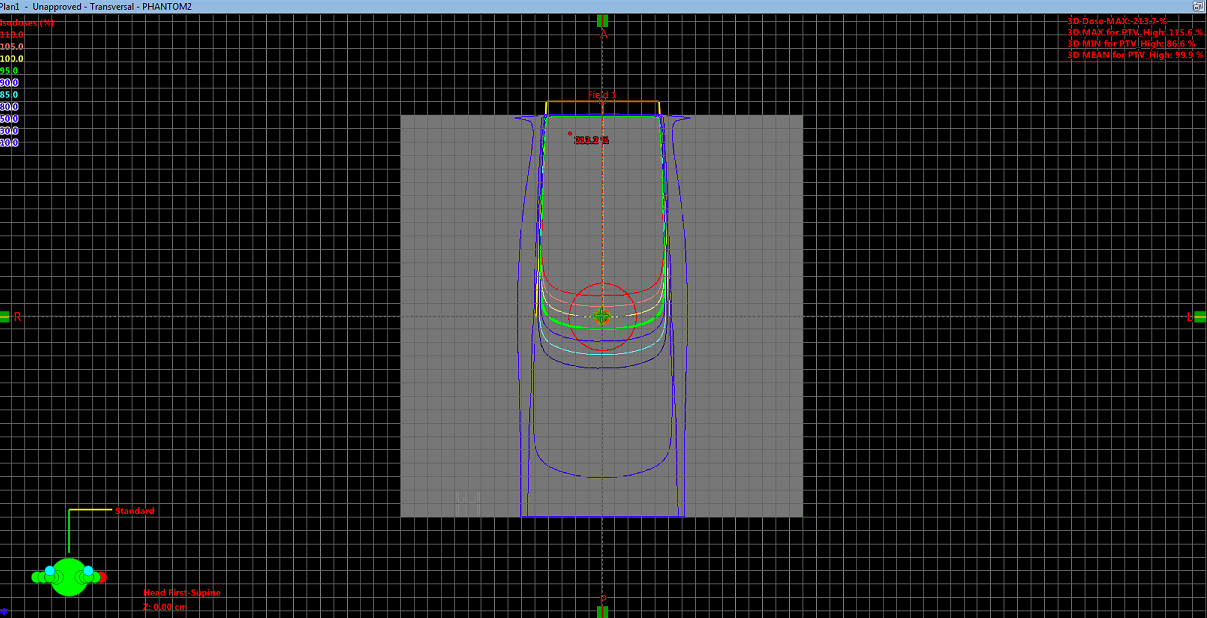
\includegraphics[width=0.9\linewidth]{../../Wasserphantom Bilder/Aufgabe2.1_2.png}
	\caption{Das Wasserphantom und das bestrahlte Feld mit einem Grid von $\SI{1}{\centi\meter}$.}
	\label{fig:aufgabe21}
\end{figure}

Für die Darstellung der Dosisverteilung im Phantom, wird ein Querprofil erstellt. Es wird in diesem Fall senkrecht zum Zentralstrahl in einem Bild aufgenommen. Dies ist in der Abbildung \ref{fig:aufgabe2} zu sehen. Aus dieser Abbildung kann entnommen werden, dass am Rand des Feldes ungefähr eine relative Dosis von $\SI{50}{\percent}$ ankommt.

\begin{figure}[H]
	\centering
	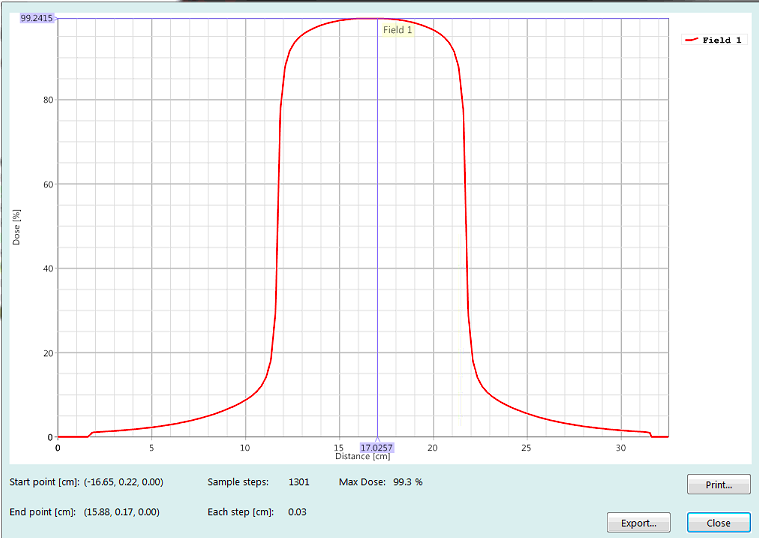
\includegraphics[width=0.7\linewidth]{../../Wasserphantom Bilder/Aufgabe213.png}
	\caption{Dosisquerprofil in der Mitte des Phantoms.}
	\label{fig:aufgabe2}
\end{figure}

Im weiteren Verlauf soll das Feld auf $\SI{6}{\centi\meter}$ x $\SI{6}{\centi\meter}$ für eine sinnvollere Bestrahlung des PTVs  verkleinert werden. Diese Dosisverteilung ist in
Abbildung \ref{fig:a2_4} dargestellt. Die Dosisberechnung zeigt, dass die $\SI{95}{\percent}$-Isodosenlinie das gesamte PTV nicht umschließt.
Der Grund dafür ist, dass die Dosisverteilung auf den Referenzpunkt, der sich im Zentrum des
PTVs befindet, normiert ist. Das bedeutet das die $\SI{100}{\percent}$-Isodosenlinie immer
durch den Referenzpunkt läuft. Da innerhalb des PTV die Strahlung weiter abgeschwächt
wird, wird hinter dem Referenzpunkt auch weniger Dosis deponiert. In diesem
Fall wird die Photonenstrahlung bereits in dem PTV so stark abgeschwächt, dass die
relative Dosis bereits in dem PTV auf unter $95\%$ absinkt.

 \begin{figure}[H]
 	\centering
 	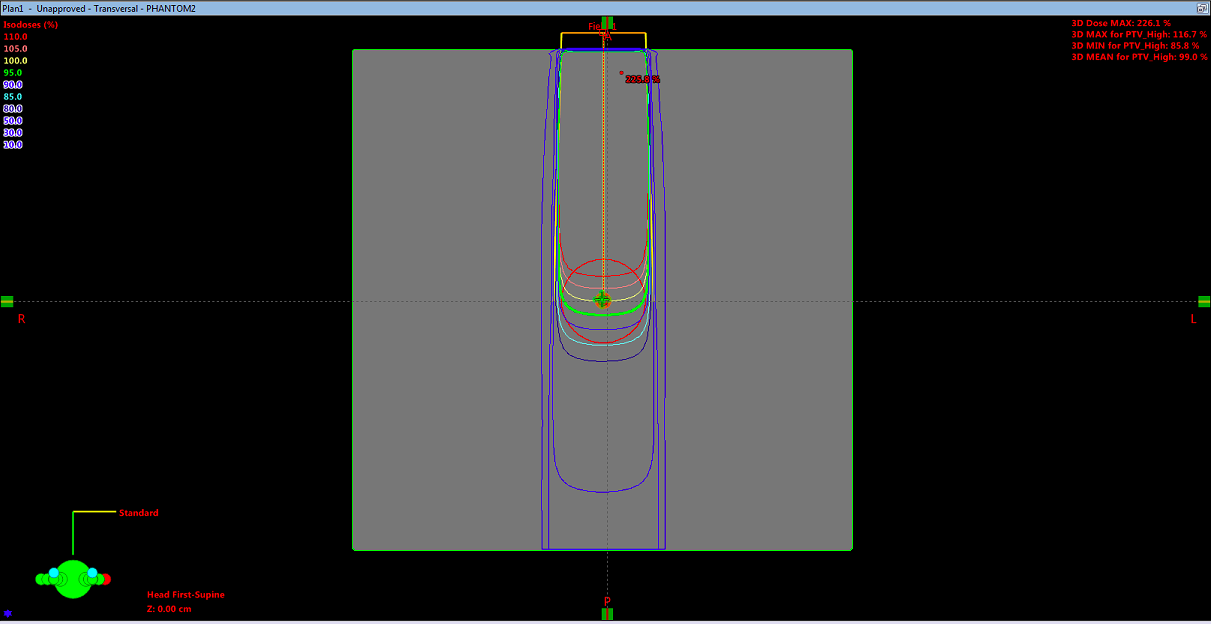
\includegraphics[width=0.7\linewidth]{../../Wasserphantom Bilder/Aufgabe2.1_4.png}
 	\caption{Dosisverteilung bei einem Strahlenfeld der Größe $\SI{6}{\centi\meter}$ x $\SI{6}{\centi\meter}$.}
 	\label{fig:a2_4}
 \end{figure}


Im letzten Schritt wird eine Tiefendosiskurve erstellt. Diese ist in Abbildung \ref{fig:aufgabe215} zu sehen wobei die Tiefendosiskurve entlang des Zentralstrahls durch das Phantom verläuft. Außerhalb des Phantoms ist keine Dosis deponiert, da dort kein Material
definiert wurde. Das bedeutet für das Programm ist außerhalb des Wasserphantoms Vakuum und
dort kann keine Dosis deponiert werden.
Innerhalb des Wasserphantoms ist der CT-Wert von Wasser eingestellt und somit wird dort
Dosis deponiert. Nach dem Eintritt der Photonenstrahlung in das Wasserphantom steigt die
Dosis zunächst an und erreicht erst in etwa $\SI{1.5}{\centi\meter}$ sein Maximum.
Das liegt an dem Dosisaufbaueffekt, der bei hochenergetischen Photonen ab etwa
$\SI{1}{\mega\eV}$ zu beobachten ist. Dieser Effekt kann mit dem Klein-Nishima-Wirkungsquerschnittes beschrieben werden, da die Wahrscheinlichkeit für Vorwärtsstreuung
mit steigender Photonenenergie zunimmt. Das bedeutet, dass bei Eintritt in das
Wasserphantom die erzeugten Sekundärelektronen und die gestreuten Photonen sich
hauptsächlich in Strahlrichtung bewegen. Durch indirekt ionisierende Photonenstrahlung
geschieht der Energieübertrag auf das Material hauptsächlich durch Sekundärelektronen und
diese bewegen sich überwiegend in Einstrahlrichtung. Die übertragene Energie und somit die Dosis
die durch die Elektronen auf das Wasserphantom übertragen wird summiert sich und wird bis
zu einem Maximum immer größer. In der Tiefe des Maximums haben die Photonen so viel Energie
abgegeben, dass die Wahrscheinlichkeit für Vorwärtsstreuung nicht mehr so groß ist.
Nach dem Maximum nimmt die deponierte Dosis also nach dem Lambert-Beerschen Gesetz exponentiell
ab. Das kann auch anhand der gemessenen Tiefendosiskurve gesehen werden. \cite{grundlagen}


\begin{figure}[H]
	\centering
	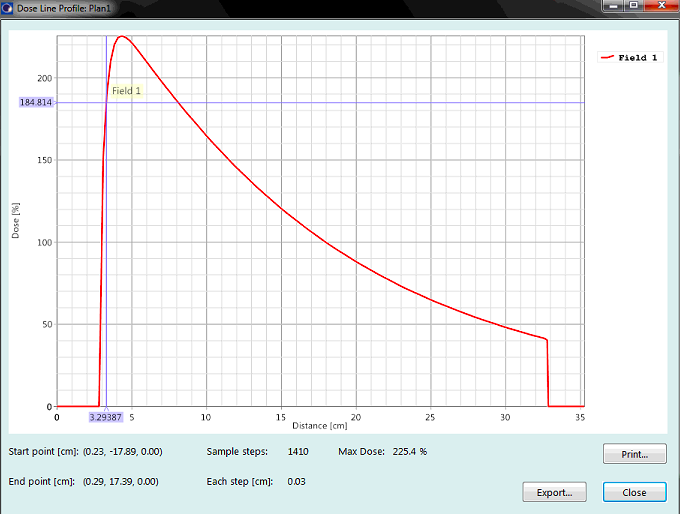
\includegraphics[width=0.7\linewidth]{../../Wasserphantom Bilder/Aufgabe215.png}
	\caption{Die Tiefendosiskurve entlang des Zentralstrahls.}
	\label{fig:aufgabe215}
\end{figure}

\subsection{4-Felder-Box}
\label{subsec:Box}

Zu dem bereit erstellten Feld werden nun drei weitere Felder erzeugt. Bei diesen
zusätzlichen Feldern sind die Gantry-Rotationen $90°$, $180°$ und $270°$. Diese haben die gleiche Eigenschaften wie das erste erstellte Feld und hierbei muss darauf geachtet werden, dass die Gesamtgewichtung bei 1 liegt. In diesem Fall hat jedes Feld eine Gewichtung von $0,25$.

\begin{figure}[H]
	\centering
	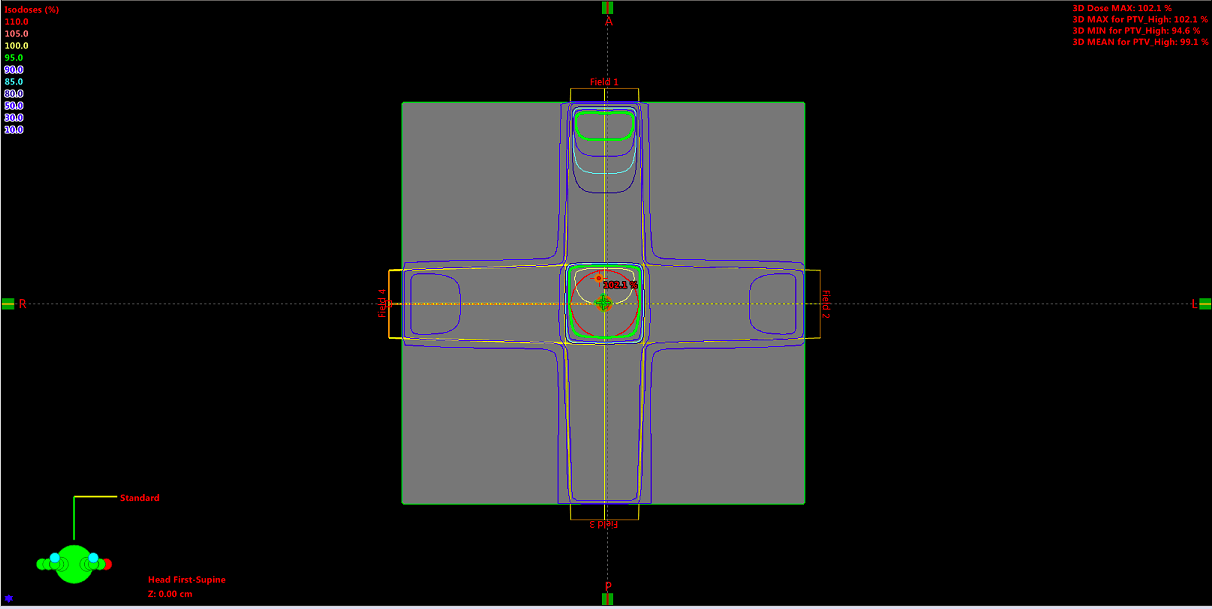
\includegraphics[width=0.7\linewidth]{../../Wasserphantom Bilder/Aufgabe222.png}
	\caption{Darstellung einer 4-Felder-Box mit einer doppelten Gewichtung eines Feldes wie die anderen drei.}
	\label{fig:aufgabe222}
\end{figure}

Danach wird eines der Felder doppelt gewichtet, wie die restlichen drei Felder. Dies ist in der Abbildung \ref{fig:aufgabe222} zu sehen. Dabei ist die Gewichtung des Feldes bei
$0°$ $40\%$ und bei den restlichen $20\%$.
Als letztes werden die Gewichtungen der Felder erneut verändert. Diesmal wird ein Feld dreifach und ein anderes doppelt so stark gewertet, wie die restlichen beiden Felder. Das ist in der Abbildung \ref{fig:aufgabe223} zu sehen. Dabei wird das Feld bei $0°$ dreifach
gewichtet also mit $42,8\%$, das Feld bei $90°$ doppelt gewichtet also mit $28,6\%$ und
die restlichen beiden Felder mit jeweils $14,3\%$.

Bei der doppelten Gewichtung eines Feldes fällt bereits auf, dass sich die Dosisverteilung
verändert. Das doppelt gewichtete Feld trägt stärker zur gesamten Dosisverteilung
als die anderen drei Felder. Somit ergibt sich eine asymmetrische Dosisverteilung
in dem PTV, obwohl die Feldanordnung symmetrisch ist.
Bei dem zweiten Beispiel ist dieses Verhalten noch besser zu sehen, da gleich zwei
Felder anders gewichtet sind. Da Feld 1 ($0°$) und Feld 2 ($90°$) stärker gewichtet
sind verläuft die $100\%$ Isodosenlinie nur im oberen und rechten Teil des PTVs
und die $95\%$ Isodosenlinie ist durch diese Gewichtung unten links besser an das PTV
angepasst. Allerdings wird durch die starke Gewichtung von Feld 1 auch außerhalb
des PTV eine hohe Dosis deponiert.
Die Variation der Feldgewichtungen könnte in der Klinik dazu verwendet werden um die
Dosisverteilung besser an das Zielvolumen anzupassen. Dadurch können auch Risikoorgane
geschont werden, wenn die Felder die zu einer Dosis in einem Risikoorgan führen
schwächer gewichtet werden.
Bei der Variation der Feldgewichtungen muss allerdings darauf geachtet werden, dass
durch eine höhere Gewichtung eines Feldes die Dosis außerhalb des Zielvolumens nicht
zu stark ansteigt, wie es in diesem Beispiel der Fall ist.

\begin{figure}[H]
	\centering
	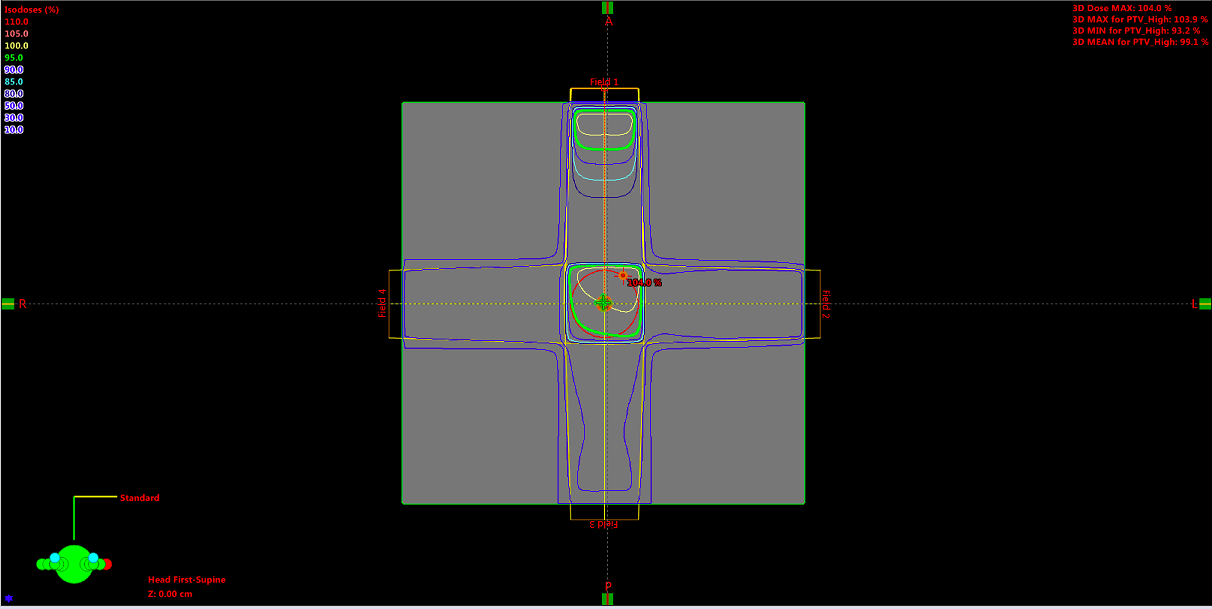
\includegraphics[width=0.7\linewidth]{../../Wasserphantom Bilder/Aufgabe223}
	\caption{Darstellung einer 4-Felder-Box mit einer dreifachen und doppelten Gewichtung wie die anderen Felder.}
	\label{fig:aufgabe223}
\end{figure}

Im letzten Teil des Abschnittes werden alle vier Felder wieder gleich gewichtet und es wird in diesem Fall wieder eine Tiefendosiskurve entlang des Zentralstrahls aufgenommen.
Diese ist in Abbildung \ref{fig:aufgabe224} dargestellt.

\begin{figure}[H]
	\centering
	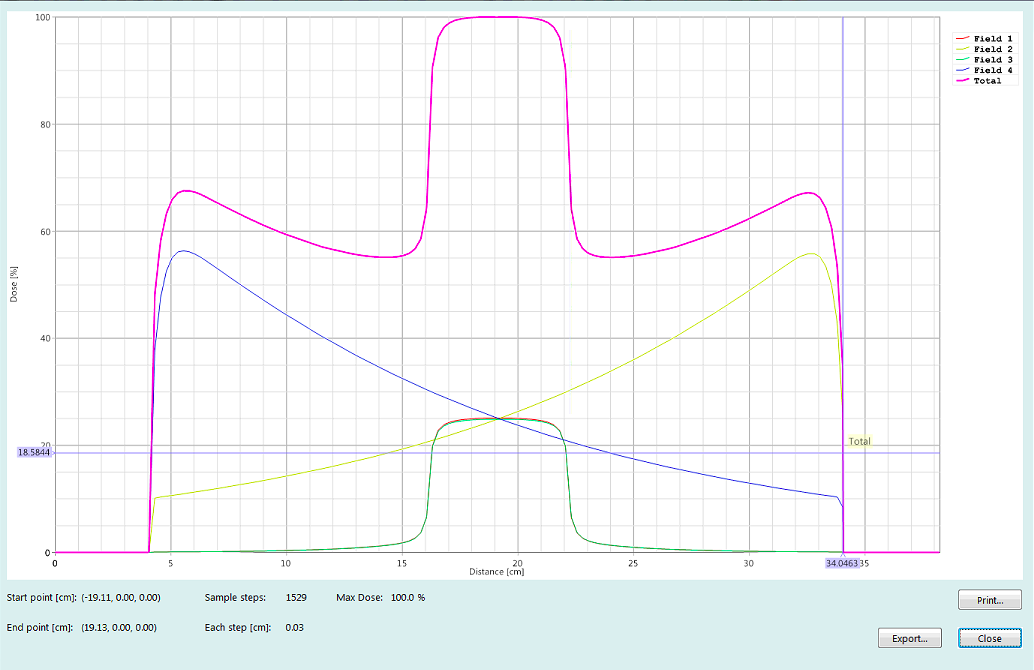
\includegraphics[width=0.7\linewidth]{../../Wasserphantom Bilder/Aufgabe224.png}
	\caption{Die Tiefendosiskurve der 4-Feldes-Box mit gleicher Gewichtung.}
	\label{fig:aufgabe224}
\end{figure}


Da in dieser Kurve vier Felder zu der Dosisverteilung in dem Wasserphantom beitragen
unterscheidet sich diese Tiefendosiskurve stark von der in Abbildung \ref{fig:aufgabe215}.
Die einzelnen Kurven von den Feldern 2 und 4 sehen ähnlich aus wie die vorher
aufgenommene Tiefendosiskurve. Das liegt daran, dass das Dosisprofil entlang
des Zentralstrahls dieser Felder aufgenommen wurde und diese beiden Felder sich
genau gegenüber liegen. Diese Kurven zeigen den gleichen Verlauf wie die vorherige
Tiefendosiskurve. Außerhalb des Wasserphantoms ist die Dosis null und bei Eintritt
in das Phantom ist ein Dosisaufbaueffekt zu erkennen. Nach dem Maximum fällt die
Dosis auch exponentiell ab.
Die einzelnen Kurven von den Feldern 1 und 3 liegen genau
übereinander und sehen ähnlich aus wie das Querprofil in Abbildung \ref{fig:aufgabe2}.
Das kommt daher, dass von diesen Feldern das Querprofil gemessen worden ist, da sie
sich auch genau gegenüber liegen und senkrecht zu den anderen beiden Feldern stehen.
Auch diese Kurven zeigen den gleichen Verlauf wie das in Abbildung \ref{fig:aufgabe2}
gezeigte Querprofil. Die Dosis steigt erst in dem Phantom etwas an. In der Mitte
des Phantoms und des PTVs, wo sich das eingestellte Feld von $\SI{6}{\centi\meter}$x
$\SI{6}{\centi\meter}$ befindet, steigt das Dosisprofil stark an bis die gewünschte
relative Dosis erreicht ist. Wenn die relative Dosis erreicht ist, ist das
Dosisprofil konstant bis die Dosis nach etwa $\SI{6}{\centi\meter}$ wieder stark abfällt.

Die gesamte Kurve (in Pink) ergibt sich aus der Summe der Dosisprofile der einzelnen
Felder. Der äußere Verlauf dieser Kurve ähnelt der Tiefendosiskurve aus Abbildung
\ref{fig:aufgabe215}, da in diesem Bereich die Felder 1 und 3 nur wenig zu
der Dosis beitragen. In der Mitte des Wasserphantoms, in dem Bereich wo die
Felder 1 und 3 hauptsächlich zu der Dosisverteilung beitragen, hat die Gesamtkurve
einen Verlauf wie in dem Querprofil in Abbildung \ref{fig:aufgabe2}. \\
Anhand des gesamten Dosisprofils ist zu erkennen, dass in der Mitte des Wasserphantoms,
dort wo sich das PTV befindet, die meiste Dosis deponiert wird.
Das ist ein Vorteil an einer Bestrahlung mit mehreren Feldern. Wird nur mit einem
Feld bestrahlt ist es durch den exponentiellen Dosisabfall schwierig eine gewünschte
Dosis in einem PTV zu erreichen, welches sich in einer gewissen Tiefe im Körper
befindet. Außerdem wird bei Verwendung eines Feldes immer die meiste Dosis bei
Eintritt in den Körper deponiert. Wie in der Abbildung \ref{fig:aufgabe224} zu sehen
ist, ist es durch Verwendung mehrerer Felder, vor allem opponierender Felder, möglich
eine maximale Dosisdeposition in einem PTV zu erreichen.
Bei der Verwendung von nur zwei opponierenden Feldern kann zwar nicht erreicht werden,
dass in dem PTV die meiste Dosis deponiert wird, allerdings kann damit eine relativ
homogene Dosisdeposition in dem im Zentrum liegenden PTV erreicht werden.
Ein Nachteil an der Verwendung von mehreren Feldern für die
Bestrahlung ist, dass dadurch die Bestrahlung länger dauert. Durch
die verschiedenen Einstrahlrichtungen und dadurch, dass das Dosismaximum der
einzelnen Felder sich kurz nach Eintritt in den Körper einstellt wird in mehr
gesunden Gewebe eine Dosis deponiert wenn mehrere Felder verwendet werden.


\subsection{Verwendung von Keilen}
\label{subsec:Keilen}

Es wird mit einem Wasserphantom und Feld analog zu Wasserphantom I gearbeitet. Zusätzlich wird hier mit Keilen gearbeitet, d.h. es wird in den Strahlengang ein Keil mit einer Stärke von 60$^\circ$ platziert. Danach soll die Dosis berechnet werden und eine DVH erstellt werden, die in der Abbildung \ref{fig:aufgabe233} zu sehen ist. Hierbei kann abgelesen werden, wie viel Prozent eines Zielvolumens mit wieviel Prozent der relativen Dosis bestrahlt werden. Zu sehen ist ein Vergleich der Bestrahlung mit Keil (Dreiecke) und ohne Keil (Quadrate). Die rote Kurve gehört zu dem PTV und die grüne Kurve zum Wasserphantom.


\begin{figure}[H]
	\centering
	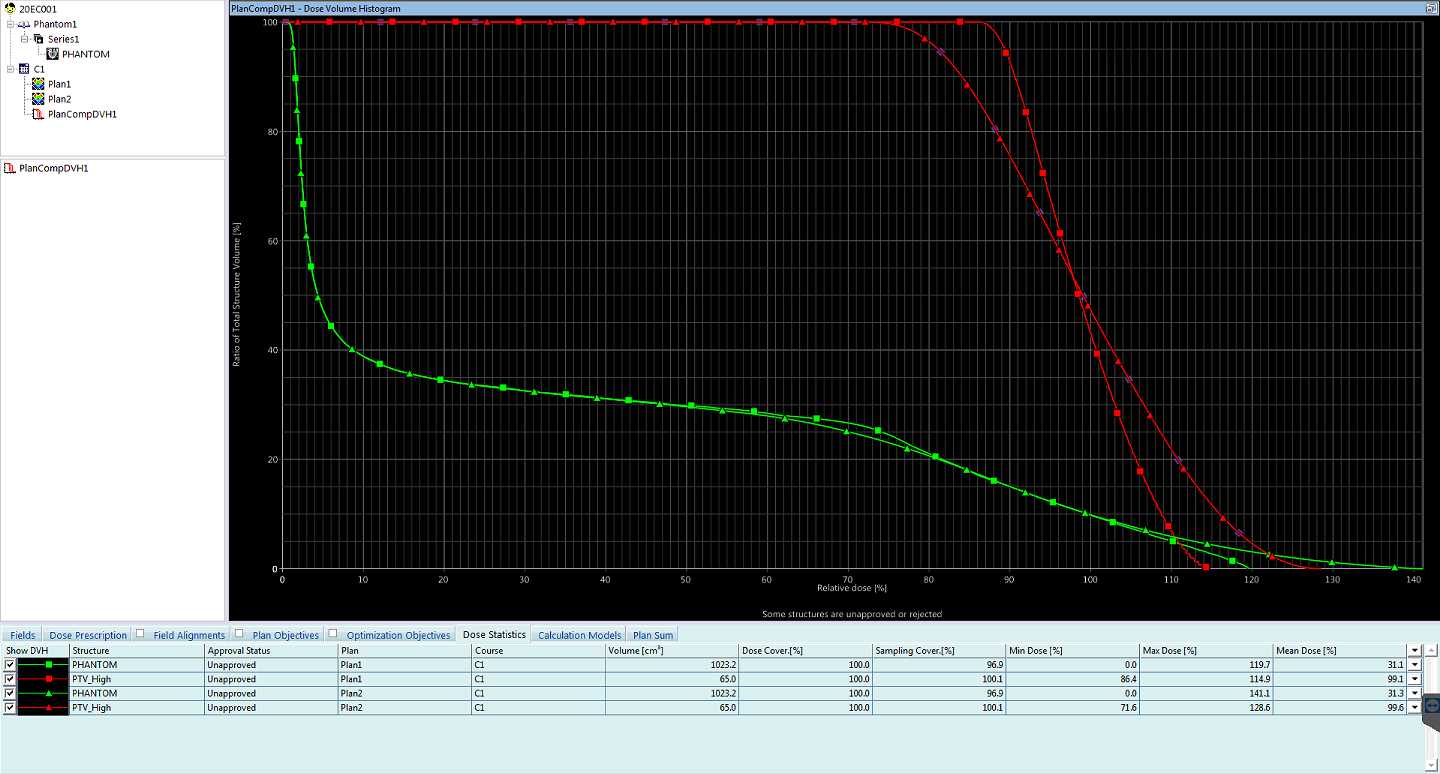
\includegraphics[width=0.7\linewidth]{../../Wasserphantom Bilder/Aufgabe233.png}
	\caption{Das DVH mit Keil (Dreiecke) und ohne Keil (Quadrate) des Wasserphantoms in grün und des PTVs in rot.}
	\label{fig:aufgabe233}
\end{figure}

Zu beobachten ist, dass bei der Verwendung eines Keilfilters die maximale
relative Dosis bei der Bestrahlung höher ist als ohne den Filter. Anhand
der roten Kurve ist zu erkennen, dass die Dosisdeposition in dem PTV bei der
Verwendung eines Keilfilters inhomogener ist als ohne den Filter. Das
liegt daran, da das Strahlenfeld durch den Keilfilter beeinflusst wird und somit
die Dosisverteilung in dem PTV und auch im gesamten Wasserphantom asymmetrisch
wird.

Im weiteren Verlauf sollen zwei neue Pläne am gleichen Wasserphantom erstellt werden.
Dabei werden zwei opponierende Felder mit Gantry Rotationen von 0$^\circ$ und 180$^\circ$ mit einem Keilfilter der Stärke 60$^\circ$ erstellt. Hierbei muss wieder auf die Gesamtgewichtung geachtet werden. Bei einem Plan sollen die Ausrichtungen der Keile
identisch sein, diese Dosisverteilung ist in Abbildung \ref{fig:aufgabe244} zu sehen.
Bei dem zweiten Plan ist die Ausrichtung der Keile entgegengesetzt. Dieser Plan ist in
Abbildung \ref{fig:aufgabe2441} gezeigt.
Zum Vergleich der beiden Pläne wird erneut ein DVH mit den beiden Plänen erzeugt.
Dieses ist in Abbildung \ref{fig:aufgabe234} dargestellt. Dabei ist das DVH des PTVs
in rot dargestellt und das des gesamten Wasserphantoms in grün. Der Plan
mit den Keilfiltern in gleicher Ausrichtung ist durch Quadrate dargestellt und
der Plan mit den entgegengesetzen Keilfilter durch Dreiecke.

An dem DVH ist zu erkennen, dass sich die Dosisdepositionen in dem gesamten Wasserphantom
nicht unterscheiden. Das kommt daher, da es sich bei beiden Plänen um die gleichen
Felder und auch die gleichen Keilfilter handelt, die lediglich anders ausgerichtet sind.
Diese unterschiedliche Ausrichtung macht sich nur in der Dosisdeposition innerhalb
des PTVs bemerkbar, allerdings nicht wenn das gesamte Wasserphantom betrachtet wird.

Werden die zwei Kurven des PTVs betrachtet sind Unterschiede zu erkennen. Bei dem
Plan mit den entgegengesetzen Keilfiltern wird eine deutlich geringere maximale relative
Dosis deponiert als bei den anderen Plan. Der Grund dafür kann anhand der Abbildungen
\ref{fig:aufgabe244} und \ref{fig:aufgabe2441} gut gesehen werden. Bei dem ersten Plan
mit den gleichen Keilfiltern ist der Keilfilter auf der gleichen Seite am geringsten.
Aus diesem Grund verläuft die $110\%$ Isodosenlinie durch das gesamte Wasserphantom und
damit auch durch das PTV. Bei den anderen Plan sind die Keilfilter auf unterschiedlichen
Seiten am geringsten. Aus diesem Grund überlagert sich der abgeschwächte Teil des ersten
Feldes mit dem nicht abgeschwächten Teil des opponierenden zweiten Feldes und umgekehrt.
Dadurch ist die maximale Dosis in dem PTV deutlich geringer.


\begin{figure}[H]
	\centering
	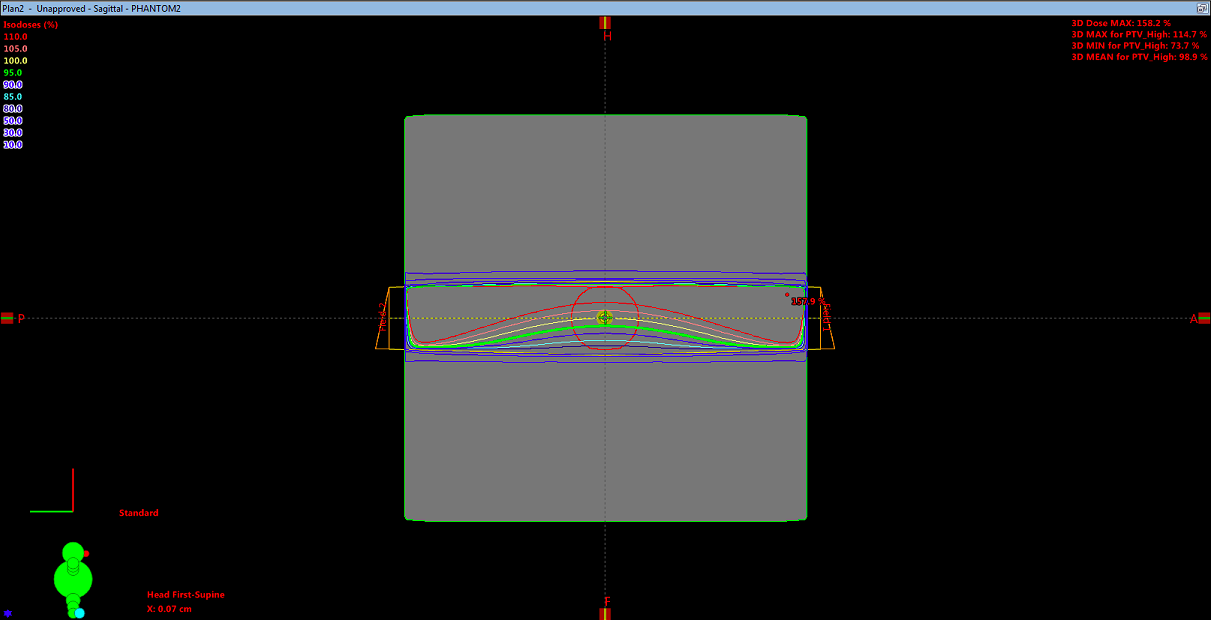
\includegraphics[width=0.7\linewidth]{../../Wasserphantom Bilder/Aufgabe244}
	\caption{Das Dosisprofil in gleicher Winkelausrichtung.}
	\label{fig:aufgabe244}
\end{figure}

\begin{figure}[H]
	\centering
	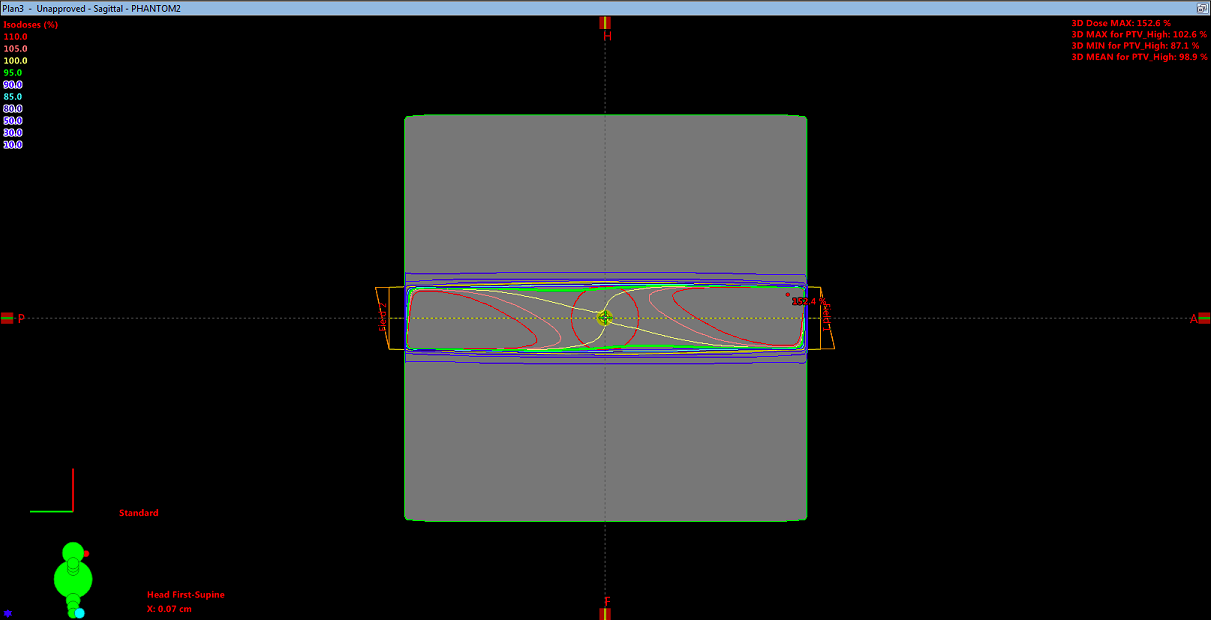
\includegraphics[width=0.7\linewidth]{../../Wasserphantom Bilder/Aufgabe2441}
	\caption{Das Dosisprofil in entgegengesetzter Winkelausrichtung.}
	\label{fig:aufgabe2441}
\end{figure}


\begin{figure}[H]
	\centering
	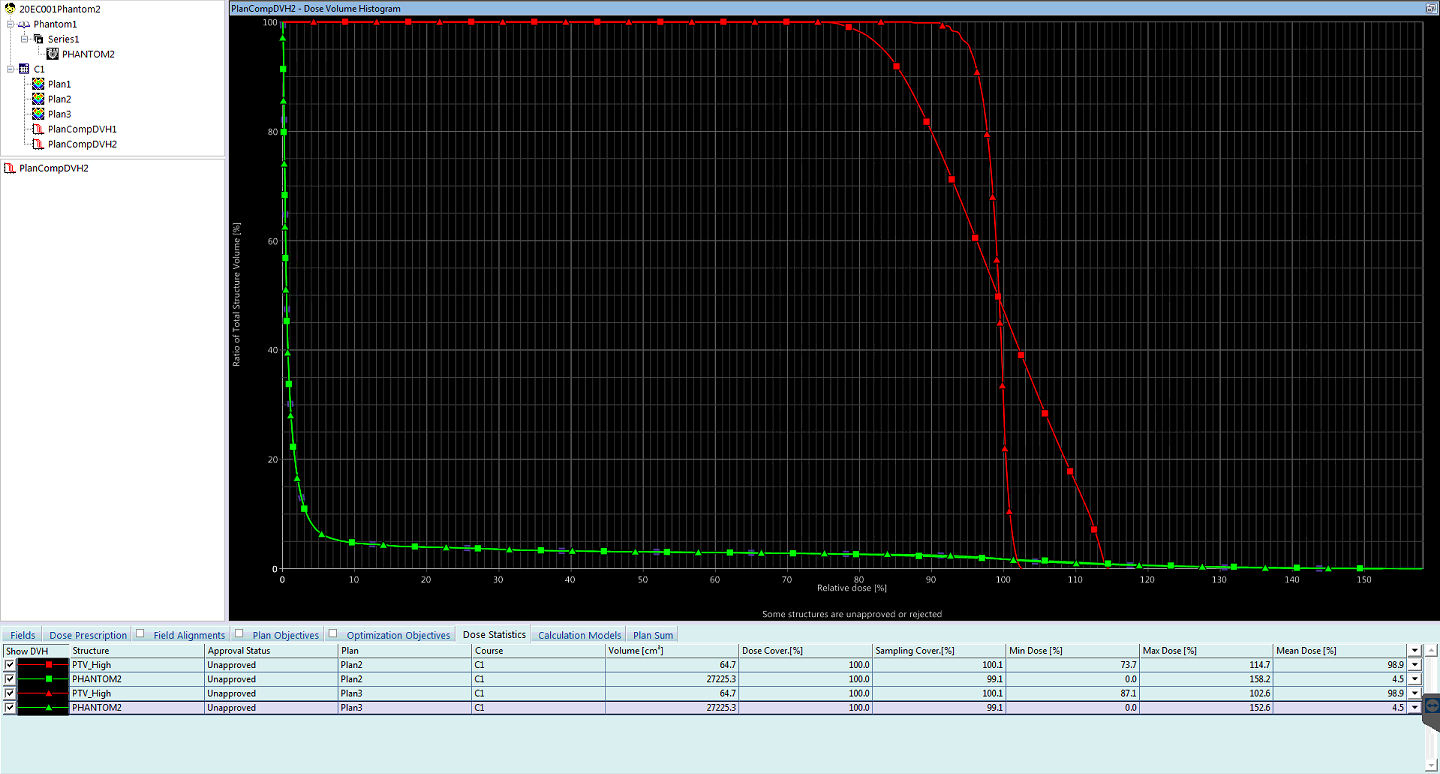
\includegraphics[width=0.7\linewidth]{../../Wasserphantom Bilder/Aufgabe234.png}
	\caption{Vergleich der beiden Dosisprofil mit Keile in selber (Quadrate) und entgegengesetze Keilen (Dreiecke) Ausrichtung des Wasserphantoms in grün und des PTVs in rot. }
	\label{fig:aufgabe234}
\end{figure}
